\section{Fundamentação de POO}

\begin{frame}{Relembrando o paradigma procedural}
  \begin{itemize}
    \item É baseado no conceito de chamada de funções por um fluxo de dados.
    \item Todas as variáveis são concentradas no fluxo de dados.
    \item As funções tomam um conjunto de variáveis como argumento e retorna o resultado para o fluxo de dados.
  \end{itemize}
  \begin{figure}
    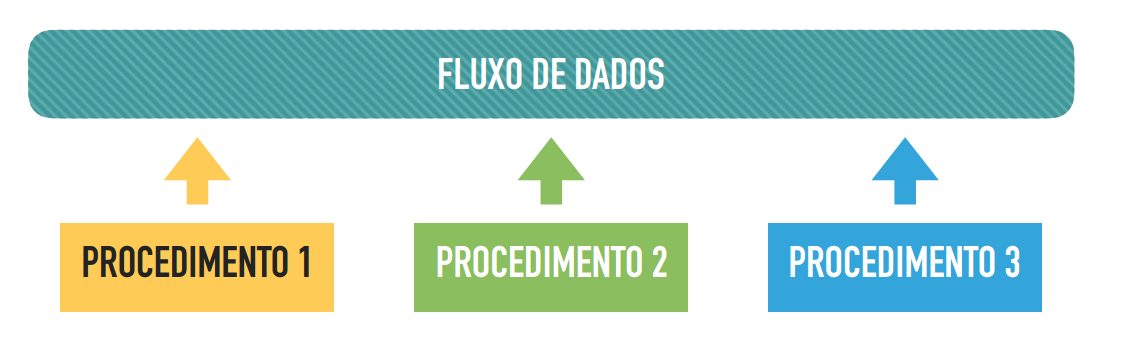
\includegraphics[width=0.85\textwidth]{figuras/fluxo.png}
    \caption{Estrutura do padadigma procedural.}
  \end{figure}
\end{frame}

\begin{frame}{Clases x Objetos}
  \begin{itemize}
    \item Uma classe é o molde especificando quais atributos (dados) e métodos (funções) os objetos criados a partir dela terão.\pause
    \item Um objeto é uma instância de uma classe, ou seja, é um individo criado a partir do molde em que é possível obter o \textbf{estado} de seus atributos. Sobre os métodos, eles são as ações que um objeto pode realizar.
  \end{itemize}
  \pause
  {\color{red}Importante}: Sobre os objetos, eles apresentam a ideia de \textbf{ciclo de vida}, eles podem ser (1) criados, (2) manipulados e (3) destruídos.
\end{frame}

\begin{frame}{O que é o paradigma OO?}
  \begin{itemize}
    \item Paradigma para desenvolvimento de software que baseia-se na noção de utilização de componentes individuais e simples (os objetos) e na comunicação (troca de mensagens) entre esse componentes para construir sistemas mais complexos.
  \end{itemize}
  \pause
  E quais as vantagens de OO?
  \begin{itemize}
    \item Facilita para reutilizar código (não reinventar a roda).
    \item A modelagem é ligeiramente aproximada, com a realidade do mundo.
    \item Pequenas mudanças nos requisitos dos sistemas não tem grandes impactos no desenvolvimento.
  \end{itemize}
\end{frame}